%HW07.tex
%Seventh Homework -- Math 629 
%
%  The percent sign is a comment character
%
%%%%%%%%%%%%%%%%%%%%%%%%%%%%%%%%%%%%%%%%%%%%%%%%%%%%%%%%%%%%%%%%%%%%%%%%%%%%%%%%%%
%
%   Look these up on line.  The first sets the type of document, and the next are for mathematics symbols, graphics and color
%
\documentclass[12pt]{article}
\usepackage{amssymb,amsmath}
\usepackage{graphicx}
\usepackage[usenames,dvipsnames,svgnames,table]{xcolor}
\usepackage{multirow}   % This is for more control over tables
%%%%%%%%%%%%%%%%%%%%%%%%%%%%%%%%  Layout     %%%%%%%%%%%%%%%%%%%%%%%%%%%%%%%%%%%%%%
\usepackage{vmargin}
\setpapersize{USletter}
\setmargrb{2cm}{1cm}{2cm}{1cm} % --- sets all four margins LTRB


%%%%%%%%%%%%%%%%%%%%%%%%%%%%%%%%%%%%%%%%%%%%%%%%%%%%%%%%%%%%%%%%%%%%%%%%%%%%%%%%%
\begin{document}
\LARGE 
\noindent
{\color{Maroon}History of Mathematics \hfill Math 629}\vspace{2pt}\\
\large
Sixth Homework: \hfill 1 March 2022\\
Due Monday 7 March 2022.
\normalsize\vspace{10pt}

To hand in: We are using Gradescope for homework submission.


\begin{enumerate}

\item  {[10]}
     Exercise 10.5.1 from Stillwell.

\item  {[10]}
     Exercise 10.6.1 from Stillwell.


\item  {[10]}
     Exercise 10.6.2 from Stillwell. 

\item  {[10]}
     Exercise 10.6.3 from Stillwell. 

 
\item  {[10]}
  Exercise 10.7.3 from Stillwell.

  For this, use the formula $\zeta(1-s) = 2 (2\pi)^{-s} \cos\frac{s\pi}{2}\,\Gamma(s)\, \zeta(s)$.
  You need to recognise the sum as $\zeta(1-s)$ and then apply this formula.  Note that for $n$ a positive integer, $\Gamma(n)=(n-1)!$.

 
\item  {[10]}
  Write a coherent few sentences (maybe a paragraph) about at least one thing that is completely wrong with the Numberphile video.
  Be sure to be mathematically correct; you may need to recall your second semester of Calculus.



\end{enumerate}

{\Large\sf\color{Maroon}Do the exercises on the other side of this page about Benford's Law.}


\newpage

{\Large Logarithms and the distribution of data (Benford's law)}


This is an experiment in the natural distribution of data.

I have made a .pdf that you can use to doodle on. It has both normally ruled and logarithmically ruled lines.
It is available from the course webpage.

\begin{enumerate}\setcounter{enumi}{6}


\item  {[10]}
    Find a list of at least 20 numbers (for example, a table of properties of the elements in a chemistry handbook). Other places to look are the population of US states, or of the countries in a particular region, or GDP or area in either square miles or hectares, areas of the world's largest lakes, stock prices, etc.
        These should be empirical data, not artificially constructed numbers such as phone numbers.
        They should span several orders of magnitude, not be tightly bunched like student GPAs.

\item  {[10]}
    Plot the numbers on a normal number line with scale 0 to 9.9999, with the first digit removed. For example: 38,133,256 with first digit removed is 8,133,256, which will get plotted as 8.133256. The distribution should be roughly uniform, since the second digit is completely random. Below is an image file that you can use if you need.


\noindent
\begin{picture}(480,45)(60,0)
 \put(0,15){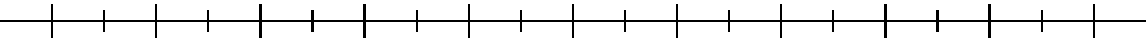
\includegraphics{TenScale}}
 \put( 22  ,0){$0$}  \put( 43,0){$0.5$}
 \put( 72  ,0){$1$}  \put( 93,0){$1.5$}
 \put(122  ,0){$2$}  \put(143,0){$2.5$}
 \put(172  ,0){$3$}  \put(193,0){$3.5$}
 \put(222  ,0){$4$}  \put(243,0){$4.5$}
 \put(272  ,0){$5$}  \put(293,0){$5.5$}
 \put(322  ,0){$6$}  \put(343,0){$6.5$}
 \put(372  ,0){$7$}  \put(393,0){$7.5$}
 \put(422  ,0){$8$}  \put(443,0){$8.5$}
 \put(472  ,0){$9$}  \put(493,0){$9.5$}
 \put(522  ,0){$10$} 
\end{picture}\vspace{20pt}




\item  {[10]}
    Plot the numbers intact (Recording the mantissa of each–this is the numerical part in scientific notation, so that 38,133,256 = 3.8133256 * 107 gets plotted as 3.88133256). You should find them strongly bunched to the low end (e.g., many more numbers begin with 1 than with 9). Below is an image file that you can use if you need.


\noindent
\begin{picture}(480,45)(60,0)
 \put(0,15){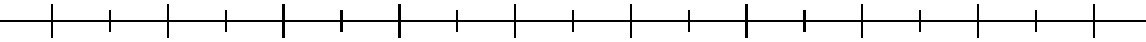
\includegraphics{NormalScale}}
 \put( 22  ,0){$1$}  \put( 44,0){$1.5$}
 \put( 77  ,0){$2$}  \put( 99.5,0){$2.5$}
 \put(133  ,0){$3$}  \put(155.5,0){$3.5$}
 \put(189  ,0){$4$}  \put(211,0){$4.5$}
 \put(245  ,0){$5$}  \put(267,0){$5.5$}
 \put(300.5,0){$6$}  \put(323,0){$6.5$}
 \put(356  ,0){$7$}  \put(378.5,0){$7.5$}
 \put(412  ,0){$8$}  \put(434,0){$8.5$}
 \put(466.5,0){$9$}  \put(490,0){$9.5$}
 \put(520  ,0){$10$} 
\end{picture}\vspace{10pt}




  \item  {[10]}
    Plot the intact numbers on a logarithmic scale. Thus you either use the log scale rule between 1 and 10, or take the logarithm of the mantissa, and plot them on normal scaled paper between 0 and 10. These two methods give the same points on the line, one should do one and not both. The distribution should now be uniform! Below is an image file that you can use if needed.



\noindent
\begin{picture}(480,45)(60,0)
 \put(0,15){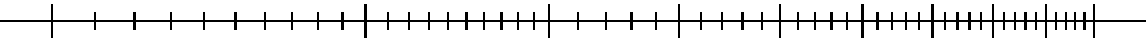
\includegraphics{LogScale}}
 \put( 21,0){$1$} 
 \put(173,0){$2$} 
 \put(261,0){$3$} 
 \put(323,0){$4$} 
 \put(372,0){$5$} 
 \put(412,0){$6$} 
 \put(445,0){$7$} 
 \put(474,0){$8$} 
 \put(500.5,0){$9$} 
 \put(520,0){$10$} 

\end{picture}\vspace{10pt}

\end{enumerate}


    This result makes sense if you think about what happens when you put the decimal point back in. The number of data points between 10 and 11 ought to be roughly the same as the number between 9 and 10, right? But if the data really span several orders of magnitude randomly, then the number between 10 and 11 should be about the same as the number between 1.0 and 1.1, and that is far fewer than the total number between 1 and 2.




\end{document}
%%%%%%%%%%%%%%%%%%%%%%%%%%%%%%%%%%%%%%%%%%%%%%%%%%%%%%%%%%%%%%%%%%%%%%%%%%%%%%%%%
